% This is the master file of the folder structure. In order to compile your document, run this file. In most LaTeX editors, the master file can be specified such that the document can also be compiled from the other .tex files (in the docs folder).

% First, the preamble needs to be called. This contains all the 'under the hood' stuff for your document.
% This file contains your LaTeX preamble. A preamble is a part of your document where all required packages and macros can be defined. This needs to be done before the \begin{document} command.

% Documentclass:
% Standard LaTeX classes are: article, book, report, slides, and letter. These cover the basis, but are not best. More advanced users might want to try out the KOMA classes or the memoir class. Optional arguments: 10pt. The font size of the main content is set to 10pt with the option between [].
\documentclass[10pt]{report}
 \usepackage[dutch]{babel}
% Geometry:
% The papersize of the document is defined with the geometry package. Here, the size is set to A4 with a4paper. Other possibilities are a5paper, b5paper, letterpaper, legalpaper and executivepaper.
\usepackage[a4paper]{geometry}

% AMS math packages:
% Required for proper math display.
\usepackage{amsmath,amsfonts,amsthm}

% Graphicx:
% If you want to include graphics in your document, the graphicx package is required.
\usepackage{graphicx}

% Booktabs:
% The booktabs package is needed for better looking tables. 
\usepackage{booktabs}

% SIunitx:
% The SIunitx package enables the \SI{}{} command. It provides an easy way of working with (SI) units.
\usepackage{siunitx}

% URL:
% Clickable URL's can be made with this package: \url{}.
\usepackage{url}

% Caption:
% For better looking captions. See caption documentation on how to change the format of the captions.
\usepackage{caption}

% Hyperref:
% This package makes all references within your document clickable. By default, these references will become boxed and colored. This is turned back to normal with the \hypersetup command below.
\usepackage{hyperref}
	\hypersetup{colorlinks=false,pdfborder=0 0 0}

% Cleveref:
% This package automatically detects the type of reference (equation, table, etc.) when the \cref{} command is used. It then adds a word in front of the reference, i.e. Fig. in front of a reference to a figure. With the \crefname{}{}{} command, these words may be changed.
\usepackage{cleveref}
	\crefname{equation}{equation}{equations}
	\crefname{figure}{figure}{figures}	
	\crefname{table}{table}{tables}
\newcommand{\projectname}{PROJECT}

% The title page is created with the command \maketitle which needs to be placed after the \begin{document} command. To create the titlepage, some entries are needed: the name of the autor is defined by \author{}, the title by the entry \title{} and the date by the command \date{}. Note that the current date is displayed with \today.
\author{Johannes Michel\\Robbert van Nijnatten\\Raymond Rohder\\Vincent Stout\\Kevin van der Vleuten}
\title{Interaction Design - \projectname}
\date{\today \\versie 1.0}

% All the actual content of your document should be placed after \begin{document} and before \end{document}. This content should be placed in the docs folder and can then be called with \input{docs/filename}.
\begin{document}

% Here the actual title page is printed, based on the given entries \author{}, \title{} and \date{}.
\maketitle

% The table of contents can be automatically generated with the \tableofcontents command. Note that you need to compile the document twice in order to see the changes in the table of contents.
\renewcommand*\contentsname{Inhoud}
\tableofcontents

% The \input{} command reads and processes the indicated example.tex file. Note that docs/ locates the folder where the .tex file is stored.
%% A chapter named 'Your first document' is created
\chapter{Your first document} \label{cha:your-first-document}


% A section called 'Basics' is created
\section{Basics} \label{sec:basics}

Text is formatted with: \textbf{bold}, \textit{italic} and \underline{underline}.
\Cref{sec:basics} is part of \cref{cha:your-first-document}.


% A subsection named 'Typesetting content' is created
\section{Typesetting content} \label{sec:typesetting}


% A subsubsection named 'Equations' is created
\subsection{Equations} \label{subsec:equations}

% Inline equations
An example of an inline equation is: the derivative of $x^2$ is $2x$. \Cref{eq:example} shows a display equation:
% Display equations
\begin{align} \label{eq:example}
          y_{0} &= \frac{\sqrt{256}}{2} \\
                &= 2^{3} = 8 \nonumber 
\end{align}


\subsection{Units} \label{subsec:units}

% % Working with units
An easy way to work with (SI) units: \SI{1}{\hertz} is equal to \SI{2\pi}{\radian\per\second}.


\subsection{Figures} \label{subsec:figures}

% Inserting a figure
Here a figure named \textit{logo.pdf} is inserted\footnote{The \textit{logo.pdf} file is located in the figs folder.}:
\begin{figure}[h]
  \centering
  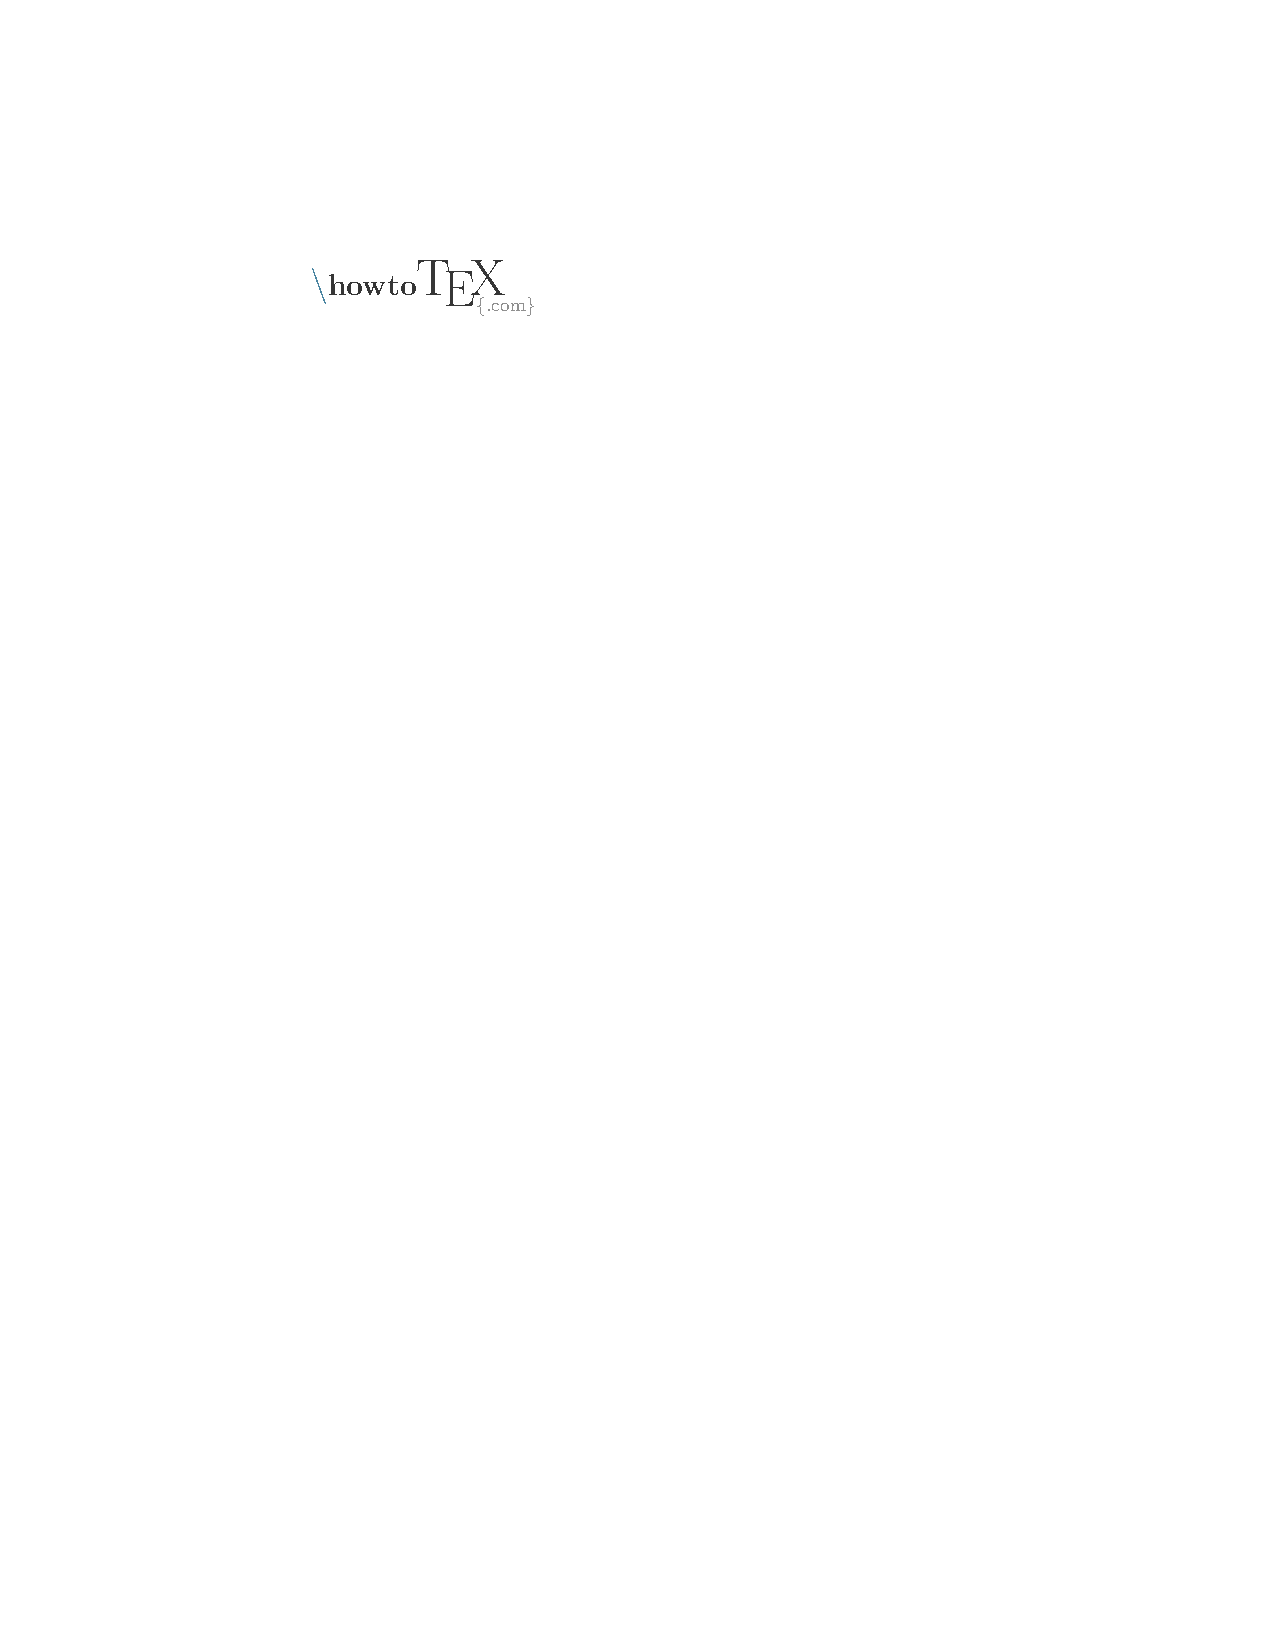
\includegraphics[width=50mm]{figs/logo}
  \caption{Caption example}
  \label{fig:logo}
\end{figure}


\subsection{Tables} \label{subsec:tables}

% Inserting a table
A table is shown in \cref{tb:table}.
\begin{table}[h]
  \centering
  \caption{Caption example}
  \label{tb:table}
  \begin{tabular}{crl}
    \toprule
    Name     & Grade & Year    \\
    \midrule
    John     & 7.5   & 2012\\
    Richard  & 2     & 2010\\
    \bottomrule
  \end{tabular}
\end{table}


\subsection{Lists} \label{subsec:lists}
% Creating lists
%% Here a subsubsection is created. Note that this section is not shown in the table of content.
\subsubsection{Numbered}
Creating a numbered list:
\begin{enumerate}
  \item First entry
  \item Second entry
\end{enumerate}

\subsubsection{Descriptive}
Creating a descriptive list:
\begin{description}
  \item[First] entry
  \item[Second] entry
\end{description}


\section{Reference to bibliography items} \label{sec:bibliography}
First are reference to a website is made \cite{MiscEntry}, then a reference to an article \cite{ArticleEntry} and finally a reference to a book \cite{last2012}.

\paragraph{Good luck!}
\chapter{Voorbereiding} \label{cha:voorbereiding}

\section{Inleiding} \label{sec:inleiding}
Project \projectname\ is een augmented reality product, in opdracht van \textit{Avans Hogeschool Breda}.

\section{Tools} \label{sec:tools}
De volgende tools zullen worden gebruikt om het interaction design van \projectname\ te realiseren.

\begin{table}[h]
  \centering
  \caption{Tools}
  \label{tb:table}
  \begin{tabular}{crl}
    \toprule
    Naam     & Type\\
    \midrule
    SketchUp     & 3D modelleer software\\
    Blender  & 3D modelleer software\\
    Adobe Photoshop & grafisch bewerkings programma\\
    LaTeX & documentatie programma\\
    \bottomrule
  \end{tabular}
\end{table}

\newpage
\section{Conceptschetsen} \label{sec:conceptschetsen}
\begin{figure}[h]
  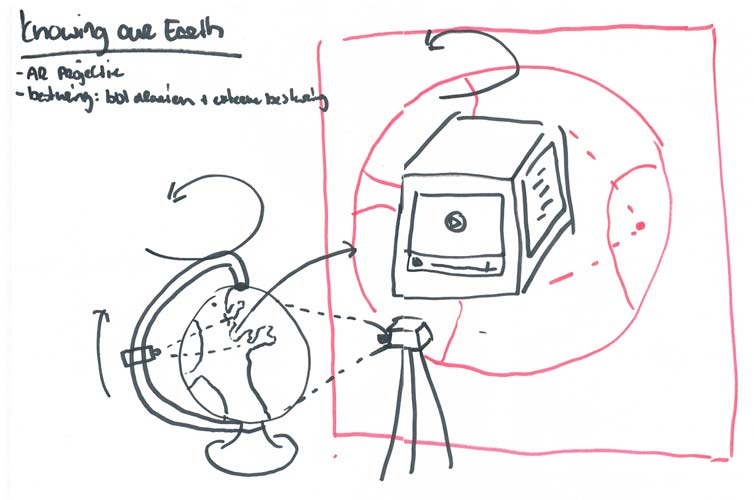
\includegraphics[width=100mm]{figs/concept1.jpg}
  \caption{Concept tekening 1 \textit{(18-April-2014)}}
  \label{fig:concept1}
\end{figure}
\begin{figure}[h]
  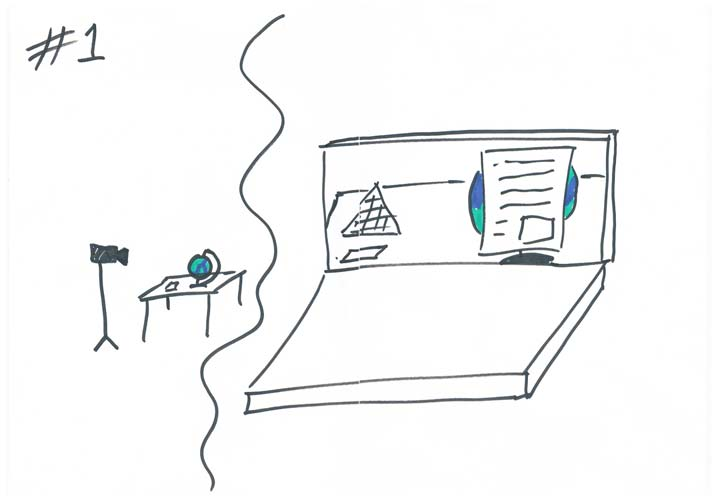
\includegraphics[width=100mm]{figs/concept2.jpg}
  \caption{Concept tekening 2 \textit{(18-April-2014)}}
  \label{fig:concept2}
\end{figure}
Weergegeven zijn de schetsen die zijn ontstaan tijdens het brainstormen over dit project. %software
\chapter{Wireframes} \label{cha:wireframes}

\section{Hoofdframe} \label{sec:hoofdframe}
\begin{figure}[h]
  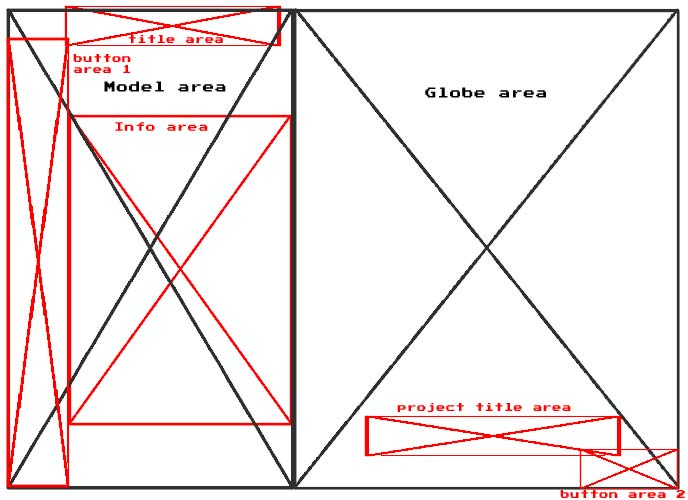
\includegraphics[width=100mm]{figs/wireframe1.jpg}
  \caption{Wireframe 1 \textit{(27-April-2014)}}
  \label{fig:wireframe1}
\end{figure}

De onderste laag is getekend in zwart, de bovenste laag is getekend in het rood.\\
De model area en globe area zijn de de belangrijkste componenten en bevatten de gehele inhoud van deze applicatie.\\
Binnen de globe area staan de project title area en de info area. De project title area is zichtbaar boven de globe area en de info area bevind zich als top laag boven alles indien zichtbaat. De project title area bevat de naam van het project, \projectname.
De inhoud van de areas zal in detail worden beschreven in \cref{cha:componenten} \nameref{cha:componenten}.
\newpage
\section{Info area wireframe} \label{sec:infowire}
\begin{figure}[h]
  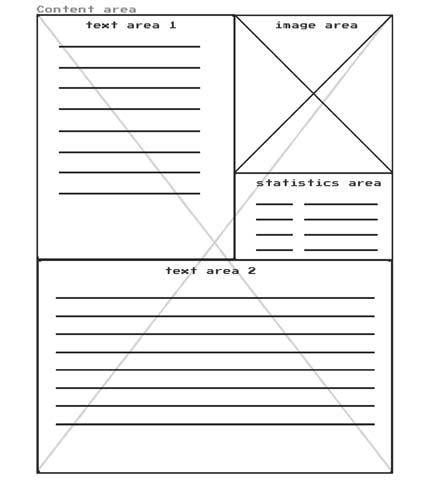
\includegraphics[width=100mm]{figs/wireframe2.jpg}
  \caption{Wireframe 2 (info area)\textit{(27-April-2014)}}
  \label{fig:wireframe2}
\end{figure}

Dit is een uitgewerkte wireframe van de info area. Dit paneel verschijnt zodra een monument wordt geselecteerd. Dit paneel kan worden gesloten met een muisklik op de knop rechtsboven in het paneel, weergegeven in het rood. In de title area staat de naam van het geselecteerde monument. In de content area komt samengevatte informatie te staan. Binnen de content area is ruimte voor text, een foto van het monument en enkele statistieken. Deze statistieken zijn gebonden aan het monument, zoals bijvoorbeeld: bouwjaar, architect en locatie gegevens. en geen ander monument kan worden gekozen terwijl het info paneel is geopend.
\newpage

% A chapter named 'Your first document' is created
\chapter{Componenten} \label{cha:componenten}


\section{Hoofdscherm} \label{sec:hoofdscherm}
\begin{figure}[h]
  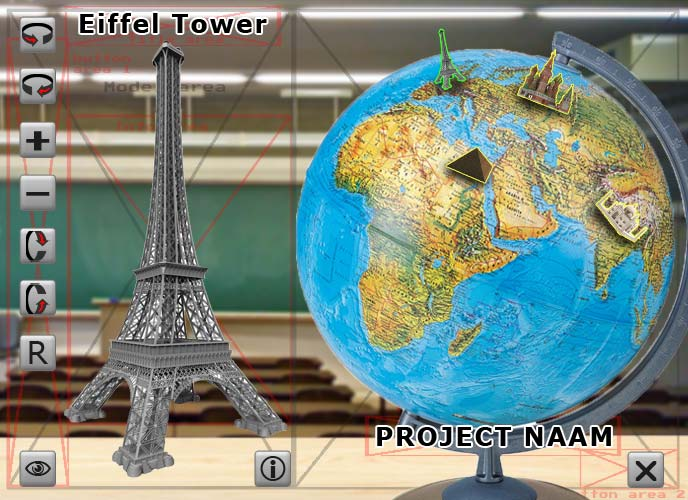
\includegraphics[width=130mm]{figs/components1.jpg}
  \caption{Componenten hoofdscherm \textit{(27-April-2014)}}
  \label{fig:components1}
\end{figure}

Het hoofdscherm is een reflectie van het camerabeeld dat wordt opgenomen. Dit scherm is wat de gebruiker hoofdzakelijk zal zien en bevat alle navigatie elementen. Het achterliggende transparante wireframe is hier slechts te zien ter verduidelijking, bij release van de applicatie zal deze niet  zichtbaar zijn. Een belangrijk aspect is dat de applicatie alleen bruikbaar is bij een specifieke wereldbol. De wereldbol is namelijk voorzien van speciale markering die dient om de positie van de 3D modellen op de bol aan te sturen.

\newpage
\section{Digitale componenten} \label{sec:digicomponents}
\begin{figure}[h]
  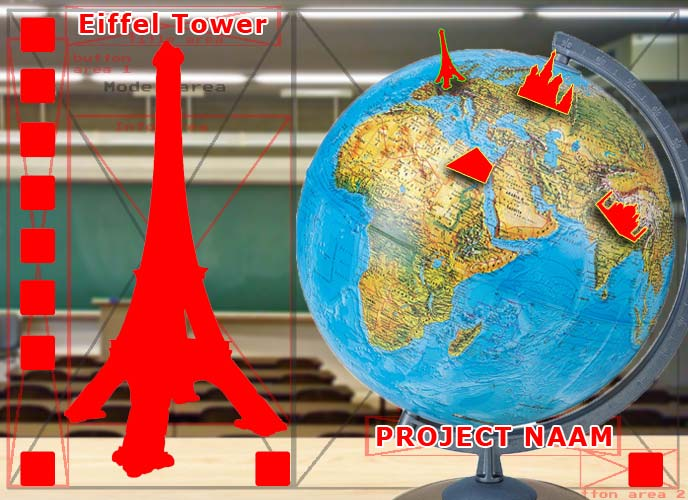
\includegraphics[width=130mm]{figs/components4.jpg}
  \caption{Digitale componenten (rood) \textit{(27-April-2014)}}
  \label{fig:digitals}
\end{figure}

In het \textbf{{\color{red}rood}} zijn alle elementen weergegeven die digitaal zullen worden weergegeven. Afhankelijk van de positie van de wereldbol zullen er 3D modellen worden weergegeven op de reflectie van de wereldbol op het scherm. Deze modellen draaien volledig mee met de assen van de wereldbol. Een geselecteerd model wordt gehighlight zodat het voor de gebruiker duidelijk is dat er iets is geselecteerd (In \cref{fig:digitals} heeft de Eiffel toren op de bol bijvoorbeeld een groene rand). 

\newpage
\section{Knoppen} \label{sec:buttons}
\begin{table}[h]
  \centering
  \caption{knoppen legenda}
  \label{tb:table}
  \begin{tabular}{crl}
    \toprule
    Button     & beschrijving   \\
    \midrule
    
\includegraphics[width=15px]{figs/button1.png}     & Pitch model rechtsom horizontaal   \\
    
\includegraphics[width=15px]{figs/button2.png}     & Pitch model linkssom horizontaal   \\
    
\includegraphics[width=15px]{figs/button3.png}     & Zoom in   \\
    
\includegraphics[width=15px]{figs/button4.png}     & Zoom uit   \\
    
\includegraphics[width=15px]{figs/button5.png}     & Yaw model naar onder   \\
    
\includegraphics[width=15px]{figs/button6.png}     & Yaw model naar boven   \\
    
\includegraphics[width=15px]{figs/button7.png}     & Reset model view   \\
    
\includegraphics[width=15px]{figs/button8.png}     & Toggle buttons aan/uit   \\
    
\includegraphics[width=15px]{figs/button9.png}     & Sluit applicatie   \\
    
\includegraphics[width=15px]{figs/button10.png}    & Toggle infoscherm aan   \\
    
\includegraphics[width=15px]{figs/button11.png}    & Toggle infoscherm uit   \\    
    \bottomrule
  \end{tabular}
\end{table}
\begin{figure}[h]
  \centering
  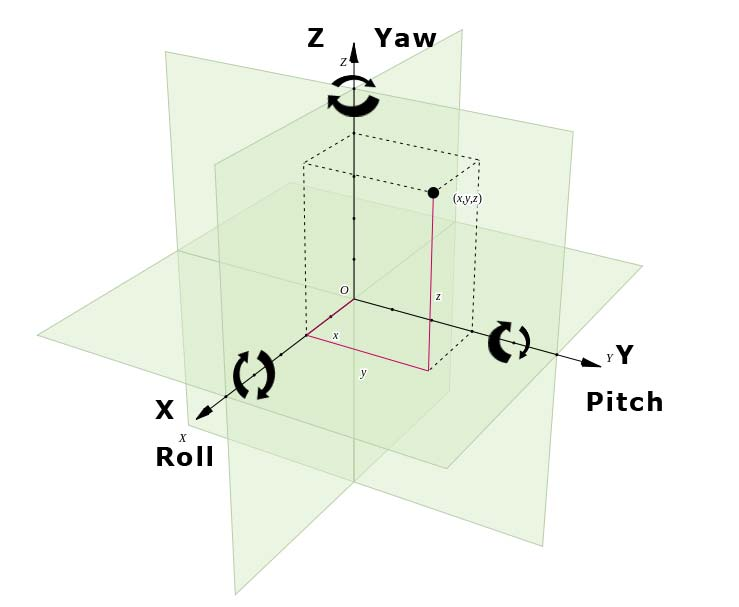
\includegraphics[width=70mm]{figs/terminology.jpg}
  \caption{XYZ axis beweging terminologie}
  \label{fig:termi}
\end{figure}

\newpage
\section{Infoscherm} \label{sec:infoscherm}
\begin{figure}[h]
  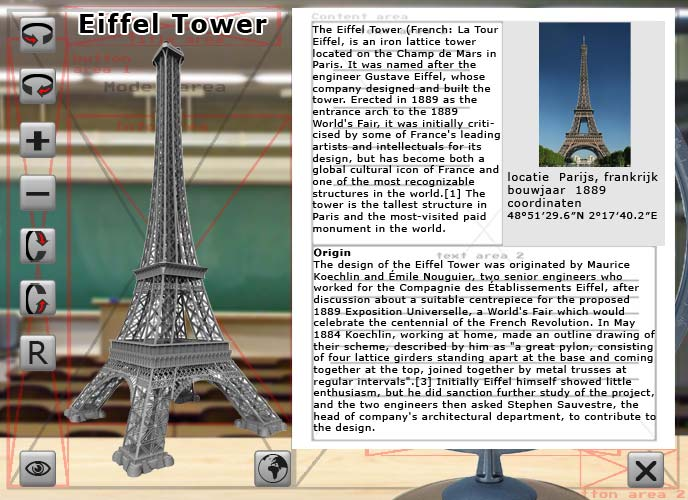
\includegraphics[width=130mm]{figs/components2.jpg}
  \caption{Componenten infoscherm \textit{(27-April-2014)}}
  \label{fig:components2}
\end{figure}
De 
\includegraphics[width=15px]{figs/button10.png} button laat een venster openen met informatie over het geselecteerde monument. Als dit scherm actief it, kan er geen monument worden geselecteerd van de wereldbol, het model links van het scherm kan nog wel worden gemanipuleerd. De gebruiker sluit het infoscherm door op de 
\includegraphics[width=15px]{figs/button11.png} button te drukken.

\newpage
\section{Afsluitscherm} \label{sec:exitscherm}
\begin{figure}[h]
  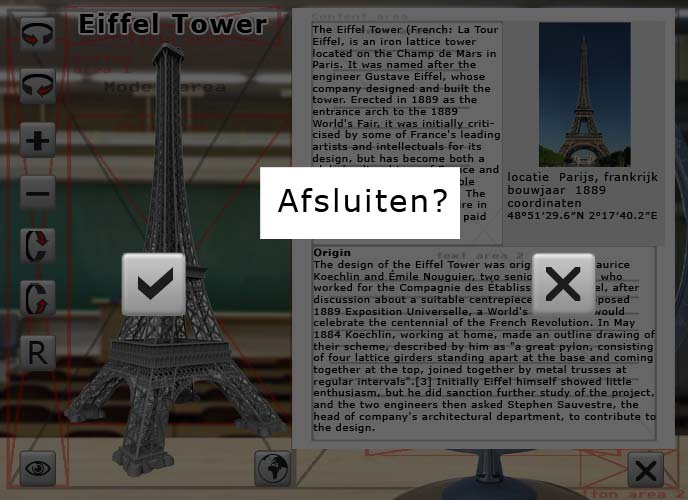
\includegraphics[width=130mm]{figs/components3.jpg}
  \caption{Componenten afsluitscherm \textit{(27-April-2014)}}
  \label{fig:components3}
\end{figure}
De gebruiker kan ten alle tijden de applicatie sluiten met de 
\includegraphics[width=15px]{figs/button9.png} button. Na het indrukken van de button verschijnt een prompt met de vraag om de applicatie te sluiten. De gehele navigatie wordt geblokkeerd zodat alleen antwoord op het prompt kan worden gegeven. De gebruiker kan kiezen om de applicatie te sluiten of terug te keren.
\chapter{User experience} \label{cha:userexperience}

\section{Basis functionaliteit} \label{sec:basis}
\projectname maakt gebruik van vision om de bewegingen van de gebruiker te registreren. De gebruiker moet daarom gemakkelijk de applicatie kunnen gebruiken met zijn/haar handen. De knoppen moeten genoeg van elkaar verspreid staan zodat er geen onhandige situaties ontstaan waarbij de gebruiker per ongeluk knoppen indrukt.\\
Dit wordt verder behandeld in \cref{sec:layout} \nameref{sec:layout}. In \cref{fig:statemachine1} staat weergegeven hoe de gebruiker navigeert door de applicatie.

\begin{figure}[h]
	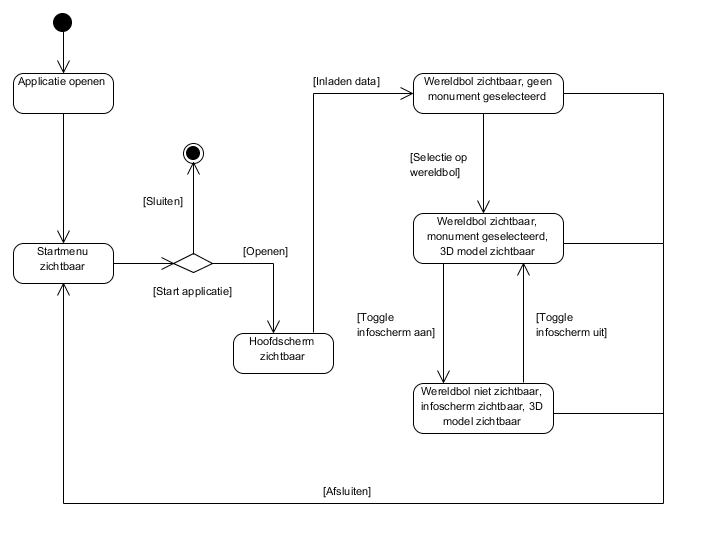
\includegraphics[width=130mm]{figs/state_machine1.png}
	\caption{State Machine diagram userflow}
	\label{fig:statemachine1}
\end{figure}


\newpage
\section{Opstelling} \label{sec:setup}
\begin{figure}[h]
	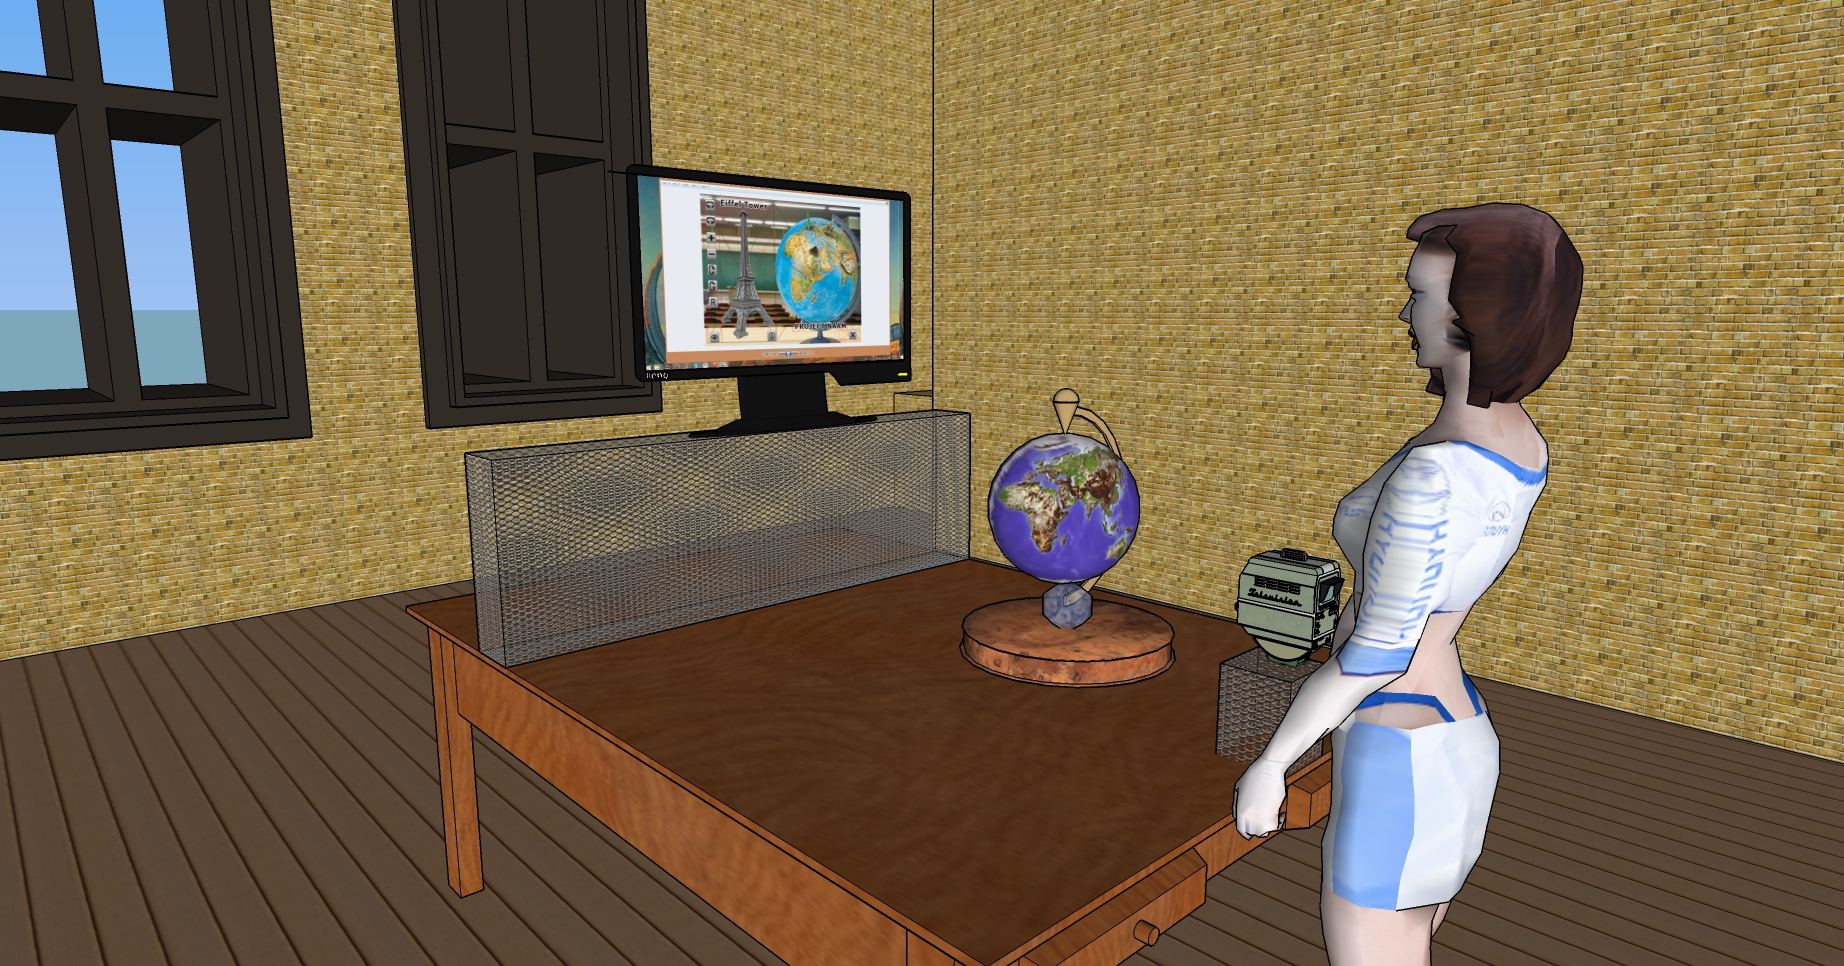
\includegraphics[width=130mm]{figs/screen1.jpg}
	\caption{Fysieke opstelling}
	\label{fig:screen1}
\end{figure}

\begin{figure}[h]
	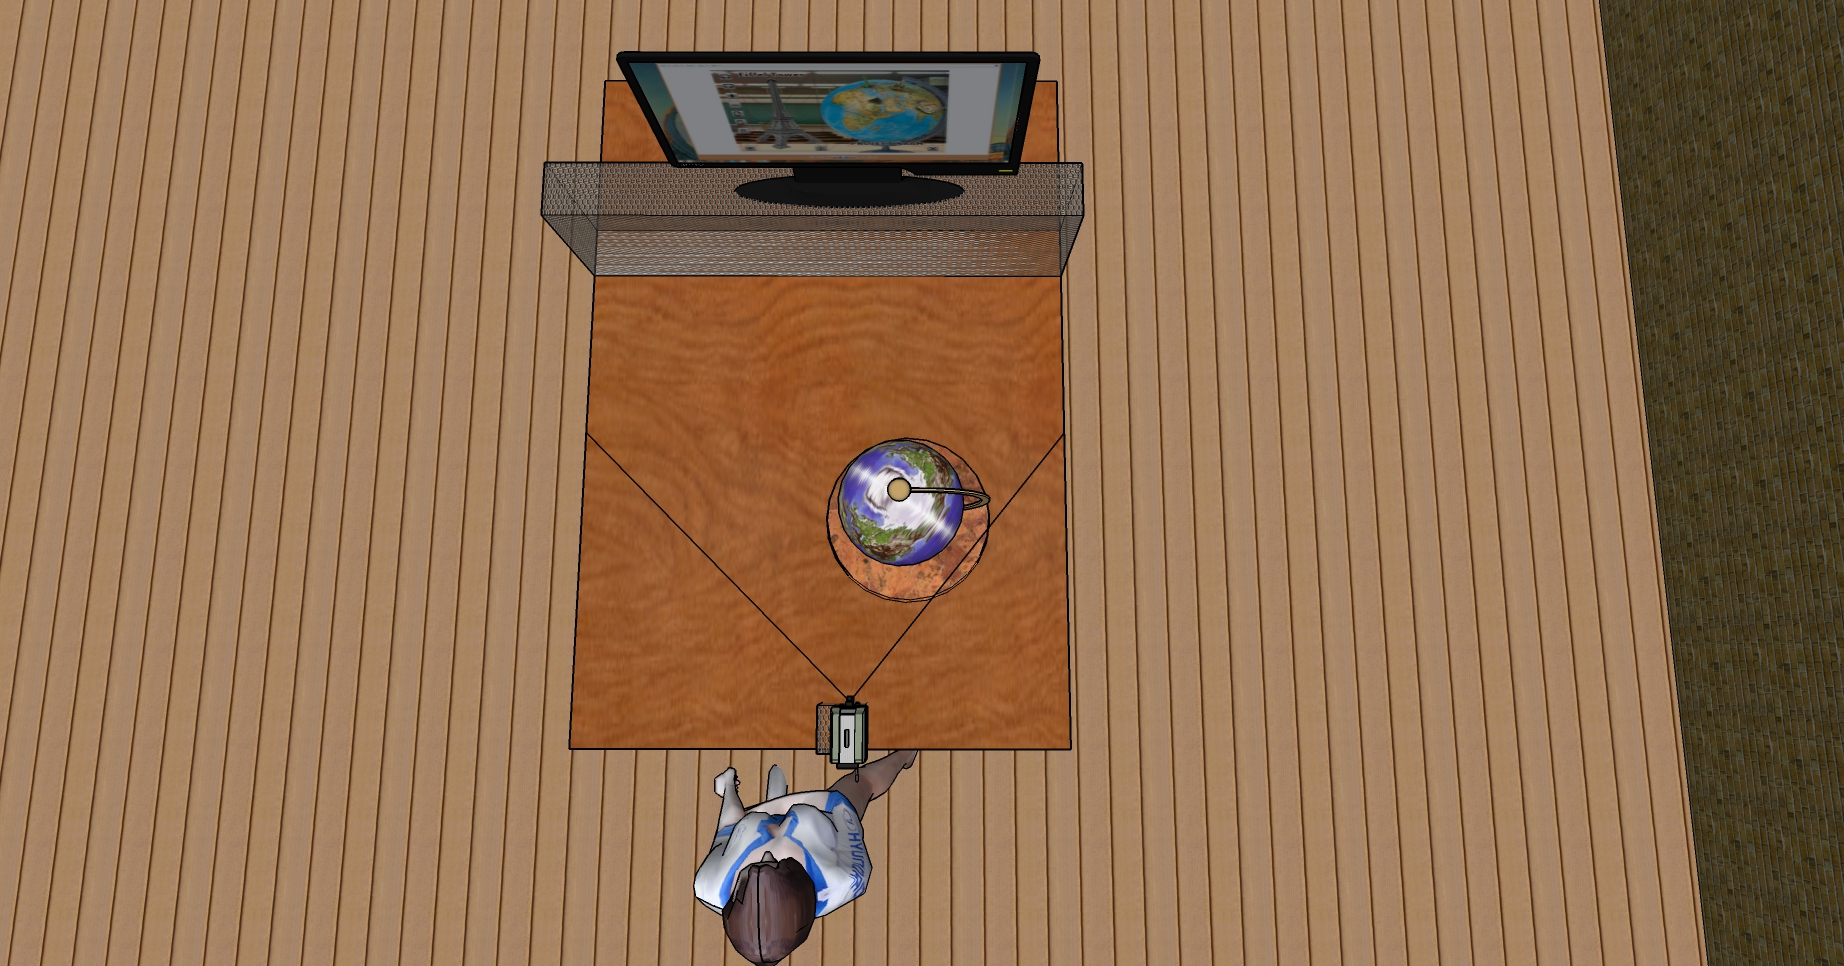
\includegraphics[width=130mm]{figs/screen2.jpg}
	\caption{Fysieke opstelling (topview)}
	\label{fig:screen2}
\end{figure}

Deze concept schetsen (\cref{fig:screen1} en \cref{fig:screen2}) geven het basis idee weer van hoe het gehele product zou moeten worden opgesteld. De camera staat op correcte hoogte om de wereldbol goed weer te geven, maar kan hinderlijk worden ervaren door de gebruiker. De wereldbol staat binnen armlengte van de gebruiker. De camera registreerd de rotatie van de wereldbol en de handen van de gebruiker. Op een computerscherm wordt de applicatie weergegeven, dit scherm wordt verhoogd naar ooghoogte van de gebruiker. Het gehele product moet ergonomisch worden ingericht, nader onderzoek zal worden gedaan naar exacte afmetingen. 

\newpage
\section{Layout} \label{sec:layout}
\begin{figure}[h]
	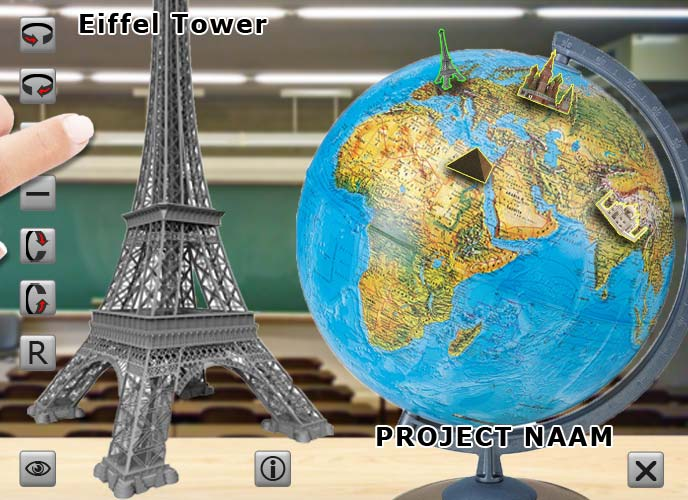
\includegraphics[width=100mm]{figs/userexp1.jpg}
	\caption{Gebruiker interactie}
	\label{fig:userexp1}
\end{figure}

De opstelling van de camera vereist van de gebruiker om zijn/haar handen om de camera heen te bewegen om zodanig de knoppen te kunnen bedienen. Deze manier van navigeren is niet geheel efficient en kan in de praktijk als onprettig worden ervaren. Om dit zoveel tegen te gaan zijn een aantal voorbereidingen getroffen.
\subsection{Knoppen margin} \label{subsec:margin}
De ruimte tussen knoppen is vergroot, zodat de kans dat de gebruiker de verkeerde knoppen indrukt verkleint. De knoppen hebben ook een offset vanaf de rand van het scherm, dit zorgt ervoor dat de gebruiker enigzins zijn/haar hand kan zien bewegen en een inschatting kan maken waar zijn/haar exacte locatie is op het scherm.
\subsection{Camera afstand} \label{subsec:cameraafstand}
De brandpuntafstand van de camera kan worden gekalibreerd zodat deze optimaal is voor zowel de hand van de gebruiker als de wereldbol. Aangezien de wereldbol binnen armlengte moet staan, kan de gebruiker dus ook met zijn/haar hand op dezelfde afstand houden. Dit zorgt voor optimale focus van de hand en de wereldbol.
\subsection{Functionliteiten schrappen} \label{subsec:scrap}
Als laatste oplossing worden bepaalde knoppen (en daarmee functionliteiten) van het scherm verwijderd om een optimalere gebruikersinteractie te krijgen. Het belangrijkste is dat de gebruiker gemakkelijk en ergonomisch de applicatie kan gebruiken. Dit betekent dus dat de layout zoals is weergegeven in dit document niet definitief is.
\chapter{Vormgeving} \label{cha:vormgeving}

De nadruk van dit project zit voornamelijk in een ergonomische layout, de vormgeving krijgt daarom geen hoge prioriteit. Dit komt door de korte periode die het ontwikkelteam krijgt om deze applicatie te bouwen en het feit dat deze weinig ervarig hebben met een soortgelijk project. Project \projectname\ kan een eigen identiteit krijgen met een logo en huisstijl, maar valt niet binnen de scope van dit project. 



% The bibliography is printed with \bibliography{}. With the command \bibliographystyle{} a style is picked.
\bibliographystyle{plain}
\bibliography{refs/references}

% To close your document, add the \end{document} command. Everything after this command will not be processed.
\end{document}
